\documentclass{article}

\input{../../../preambule}

\newtheorem{theorem}{Théorème}[subsection]

\title{Pr\'esentation d'un article : \\ On shape optimization of optical waveguides using inverse problem techniques\\\small{Thomas Felici \& Heinz W Engl}}
\author{Alexandre \bsc{Vieira}}
\date{\today}

\hypersetup{colorlinks=true, urlcolor=bleu, linkcolor=red}

\begin{document}

\maketitle
\tableofcontents

\newpage

\section*{Introduction}
Les guides d'ondes optiques sont à la base de l'optoéléctronique, ie les composants éléctroniques interagissant avec de la lumière, et de l'industrie des télécommunications. L'exemple le plus connu est bien évidemment la fibre optique, mais il existe également d'autres exemples tout aussi important, comme les composants optiques qui manipulent, filtrent et dispatchent des signaux entrants. Ces composants sont souvent de l'ordre du quart de nanomètre, ce qui représente bien sûr un avantage en poids et en volume, et qui permettent de remplir des fonctions que ne peuvent pas faire des objets plus classiques. Le développement de cette technologie repose de plus en plus sur des modèles mathématiques de paire avec des simulations numériques pour la prédiction du comportement de ces appareils, ainsi que la production d'un appareil 'optimal', ce qui repose bien souvent sur des modèles reposant sur des EDP.\\
Les adaptateurs de mode intégrés, aussi appelés "taper" en anglais, est un guide d'onde dont la section varie sur sa longueur, utilisés comme des sortes d'entonnoir. Il est bien connu que si le taper est assez long, la lumière sera transmise sans perte d'énergie. Mais plus la longueur est courte, plus le faisceau perd en énergie. Le but de ce papier était donc de trouver une formulation pour minimiser la perte d'énergie pour une longueur donnée.\\
Dans un premier temps, l'article met en place un premier problème direct pour la propagation d'une onde éléctromagnétique à traver un guide d'onde, puis il définit le problème d'optimisation. Comme on le vera, on peut ensuite dériver de ce modèle une formulation pour les modes, et établir des équations d'évolution pour l'excitation des modes dans le taper. Une problème d'optimisation en dimension finie basée sur une discrétisation sortira enfin de tout cela. \\
Des exemples numériques basés sur cette méthode montre que si la discrétisation devient trop fine, la convergence ralentit et la solution devient de plus en plus instable. Le problème vient du fait qur le problème d'optimisation est mal posé. L'article présente donc une méthode pour maximiser l'énergie résultante basée sur un problème inverse non linéaire, ainsi que des résultats numériques coroborant leur idée. 

\section{Formulation du problème direct en 2D}
\subsection{Dérivation des équations}
Les équations homogènes de Maxwell dans un milieu continu avec la permitivité linéaire $\varepsilon$ et la perméabilité magnétique $\mu_0$ sont :
\begin{equation}\label{MaxEq}
\begin{array}{c c c}
	\nabla\wedge H&=& \varepsilon\dot{E}\\
	\nabla\wedge E&=& -\mu_0\dot{H}\\
	\nabla\bullet(\varepsilon E)&=&\nabla\bullet H=0
\end{array}
\end{equation}
On se concentre uniquement sur le cas 2D. On assume donc que $E$ et $H$ sont indépendants de $y$. Si on assume une dépendance périodique en temps $e^{-i\omega t}$ et qu'on note $E=(E_x,E_y,E_z)$ et $H=(H_x,H_y,H_z)$ les composantes spatiales de la solution, on a une solution avec $H_y=E_x=E_z=0$ - le champ TE (transverse electric) - vérifiant :
\begin{equation} \label{eq2}
\begin{array}{c c c}
	\frac{\partial H_x}{\partial z} - \frac{\partial H_z}{\partial x}&=&-i\omega\varepsilon E_y\\
	\frac{\partial E_y}{\partial z}&=&-i\omega\mu_0H_x\\
	\frac{\partial E_y}{\partial x}&=&i\omega\mu_0  H_z
\end{array}
\end{equation}

En redérivant les deux dernières équations de (\ref{eq2}) par rapport à respectivement $z$ et $x$ et en réintroduisant le résultat dans la première équation, on obtient l'équation d'Helmholtz pour $E_y$ :
\[ \Delta E_y + k^2n^2E_y = 0 \text{ avec } \omega\sqrt{\mu_0\varepsilon_0}=k \text{ et } n^2=\frac{\varepsilon}{\varepsilon_0} \]
où $\varepsilon_0$ désigne la permitivité du vide.

On remarque également qu'on obtient une solution avec $E_y=H_x=H_z=0$ -le champ magnétique transverse ('TM') - donnant une équation légèrement modifiée :
	\[-\Delta H_y+k^2n^2H_y=0\]

Cependant, l'analyse ne se poursuivra qu'avec les modes du champ TE.

\bigskip
\begin{figure}[!h]
	\centering
	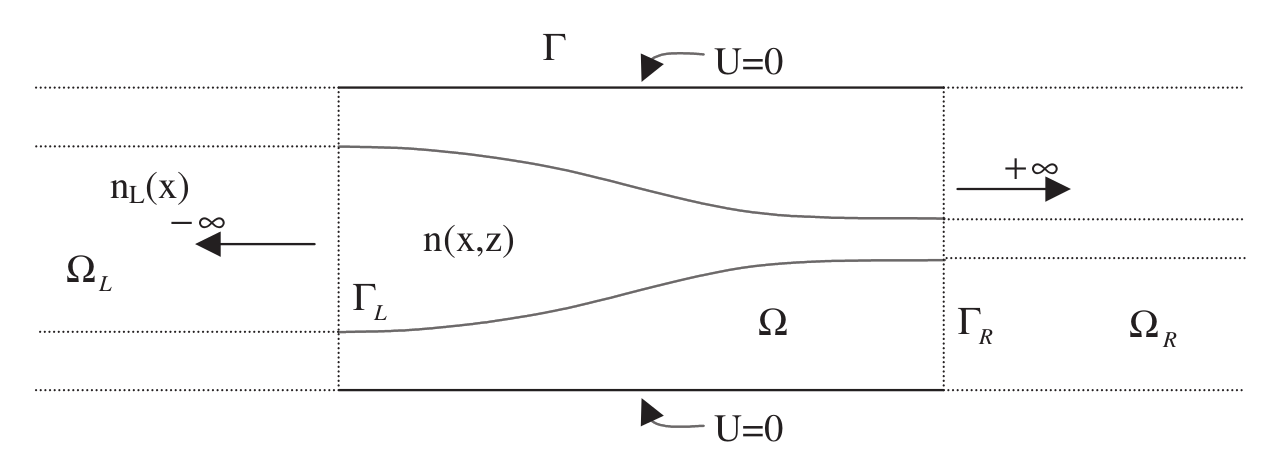
\includegraphics[scale=0.35]{images/waveguide-Taper.png}
	\caption{Profil du taper}
	\label{fig:Profil}
\end{figure}
Nous allons maintenant formuler le problème de propagation de l'onde dans un guide d'onde générique $\Omega$ en notant la frontière $\Gamma\cup\Gamma_R\cup\Gamma_L$ (voir la figure \ref{fig:Profil}).\\
À présent, pour plus de commodité, $E_y$ sera noté $U$. Sur le bord $\Gamma$, nous prenons des conditions de Dirichlet ($U=0$). Physiquement, cela signifie que le champ est réfléchi vers $\Omega$. En pratique, cela n'est pas un problème si on cherche des solutions de champs guidés, car ils sont par définition limités au guide d'onde et décroissent exponentiellement en dehors (ce qui sera discuté plus en détail ultérieurement). On réécrit donc les équations :
\begin{eqnarray}
	\label{eq3} \Delta U + n^2U&=&0 \text{ pour } (x,z)\in\Omega\\
	\label{eq4} \restriction{U}{\Gamma}&=&0
\end{eqnarray}
où on a posé $k=1$. Cela n'est rien d'autre qu'une normalisation de l'équation : on pose simplement $x'=kx$ et $z'=kz$. Ainsi : 
	\[(\partial^2_x+\partial^2_z)U(x',z')=k^2 (\partial^2_{x'}+\partial^2_{z'})U(x',z')=k^2\Delta U(x',z')\]
D'où :
	\[k^2\Delta U + n^2k^2 U =0\]
On obtient l'équation précédente en simplifiant par $k^2$.

\bigskip
Nous avons besoin à présent de conditions à $\pm\infty$. Nous prenons comme hypothèse que nous avons un champ entrant venant de $-\infty$. Ce champ $U_I$ satisfait également (\ref{eq3}), (\ref{eq4}) dans $\Omega_L$. Nous devons retrouver le fait que le champ diffusé $U-U_I$ voyage vers l'extérieur des deux côtés du guide d'onde. Nous allons faire cela en terme de modes propres dans $\Omega_L$ et $\Omega_R$, ce qui amène donc à considérer un problème spectral dans ces régions.\\
Dans $\Omega_L$, on prend une dépendance périodique par rapport à $z$ : $U(x,z)=\tilde{U}(x)e^{i\beta z}$. En réinjectant cela dans (\ref{eq3}), on obtient :
\begin{equation}\label{eq5} \frac{d^2\tilde{U}}{dx^2} + (n^2-\beta^2)\tilde{U}=0 \text{ pour un } z \text{ fixé avec } \tilde{U}(x_{min})=\tilde{U}(x_{max})=0 \end{equation}

Les conditions de Dirichlet (\ref{eq4}) nous assure que nous avons en ensemble de valeurs propres discrètes $\{(\tilde{U}_k,\pm\beta_k):k\in\mathbb{N}^*\}$. On a donc :
\begin{equation}\label{eq6} U(x,z)=\sum_{k=1}^\infty \left(C_ke^{i\beta_k z}+C_{-k}e^{-i\beta_k z}\right) \tilde{U}_k(x) \text{ dans } \Omega_L \end{equation}

Notons que le raisonnement tient toujours dans $\Omega_R$ et donne un résultat similaire.\\
Dans (\ref{eq6}), on pose $\beta_k>0$ si $\beta_k$ est réel, $\beta_k=i|\beta_k|$ si $\beta_k$ est imaginaire. Ainsi, les coefficients $C_k$ et $C_{-k}$ représentent respectivement le voyage vers la droite et vers la gauche de l'onde.\\
De plus, on remarque que l'opérateur utilisé dans (\ref{eq3}) est auto-adjoint pour le produit scalaire $\langle a,b\rangle = \int_{x_{min}}^{x_{max}} a(x)b(x)dx$. En effet :
\begin{eqnarray*}
\left\langle (\Delta +n^2 Id)u,v\right\rangle&=&\langle \Delta u,v\rangle + \langle n^2u,v\rangle \\
					&=&\int_{x_{min}}^{x_{max}} \Delta u(x) v(x) dx + \langle u,n^2 v \rangle \\
					&=&-\int_{x_{min}}^{x_{max}} \nabla u(x). \nabla v(x) dx + \underbrace{\left[\nabla u(x).n v(x)\right]_{x_{min}}^{x_{max}}}_{=0 \text{ dû au conditions de Dirichlet}}+ \langle u,n^2 v \rangle \\
					&=& \int_{x_{min}}^{x_{max}} u(x) \Delta v(x) dx - \underbrace{\left[\nabla v(x).n u(x)\right]_{x_{min}}^{x_{max}}}_{=0} + \langle u,n^2 v \rangle \\
					&=& \left\langle u,(\Delta +n^2 Id)v\right\rangle
\end{eqnarray*}

Cela assure ainsi que les modes propres sont orthogonaux relativement à ce produit scalaire. De plus, si on normalise les normes :
\begin{equation} \label{eq7} \langle \tilde{U}_k,\tilde{U}_k\rangle = \frac{1}{\beta_k} \end{equation}
la puissance transmise dans chaque mode propre $k$ est donné par $|C_k|^2$.\\
Étant donné cette normalisation, une onde sortante $U_L$ (vers $-\infty$) est donnée en posant $C_k=0$ pour tout $k>0$. Ainsi :
\begin{eqnarray*}
\beta_k\langle U_L,\tilde{U}_k\rangle &=&\beta_k\sum_{j=1}^\infty C_{-j}e^{-i\beta_j z}\langle \tilde{U}_j,\tilde{U}_k \rangle \\
				      &=&\beta_k C_{-k} e^{-i\beta_k z} \frac{1}{\beta_k}\\
				      &=&C_{-k} e^{-i\beta_k z}
\end{eqnarray*}

De même, une onde entrante $U_I$ est donnée en fixant $C_{-k}=0$ pour tout $k>0$ et $C_k$ est donné par \[C_ke^{i\beta_k z}=\beta_k\langle U_I,\tilde{U}_k\rangle\]
Enfin, on différencie (\ref{eq6}) pour $U_L$ et $U_I$ pour obtenir les conditions au bord sur les côtés. On obtient ainsi :
\[\frac{\partial U_L}{\partial z} =\sum_{k=1}^\infty -i \beta_k C_{-k} e^{-i\beta_k z} \tilde{U}_k(x)\]
\begin{equation} \label{eq8} 
\frac{\partial U_L}{\partial z}= -i \sum_{k=1}^\infty \beta_k^2 \langle U_L,\tilde{U}_k\rangle \tilde{U}_k(x) \text{ dans }\Omega_L\text{ - condition pour les ondes partant vers }-\infty
\end{equation}
De même : 
\begin{equation} \label{eq9} 
\frac{\partial U_I}{\partial z}= -i \sum_{k=1}^\infty \beta_k^2 \langle U_I,\tilde{U}_k\rangle \tilde{U}_k(x) \text{ dans }\Omega_L\text{ - condition pour les ondes venant de }-\infty
\end{equation}

Puisque $U=U_I+U_L$, en replaçant $U_L$ dans (\ref{eq8}) et en utilisant (\ref{eq9}), on obtient : 
	\[\frac{\partial U}{\partial z}=-i\sum_{k=1}^\infty {\beta_k^{(L)}}^2\left\langle U,\tilde{U}^{(L)}_k\right\rangle \tilde{U}^{(L)}_k + 2i\sum_{k=1}^\infty {\beta_k^{(L)}}^2 \left\langle U_I,\tilde{U}_k^{(L)}\right\rangle\tilde{U}^{(L)}_k \]
En surmontant le tout de l'exposant $(L)$ pour indiquer que le tout vient de la gauche, ie de $-\infty$.\\
De même, pour les ondes se propageant vers $+\infty$, et en supposant qu'il n'y a aucune onde venant de là, on obtient :
\[\frac{\partial U}{\partial z}=i\sum_{k=1}^\infty {\beta_k^{(R)}}^2 \left\langle U,\tilde{U}_k^{(R)} \right\rangle \tilde{U}_k^{(R)} \text{ dans } \Omega_R \text{ - condition pour les ondes allant vers }+\infty\]
Le problème complet est donc : trouver $U(x,z)$ tel que : 
\begin{equation} \label{eq10}
\left\{\begin{array}{r c l r}
	\Delta U + n^2U&=&0 &\text{pour } (x,z)\in\Omega\\
	\restriction{U}{\Gamma}&=&0 &\text{(murs réfléchissants)}\\
	\frac{\partial U}{\partial z}+i\sum_{k=1}^\infty {\beta_k^{(L)}}^2\left\langle U,\tilde{U}^{(L)}_k\right\rangle \tilde{U}^{(L)}_k &=& 2i\sum_{k=1}^\infty {\beta_k^{(L)}}^2 \left\langle U_I,\tilde{U}_k^{(L)}\right\rangle\tilde{U}^{(L)}_k &\text{sur }\Gamma_L\\
	\frac{\partial U}{\partial z}-i\sum_{k=1}^\infty {\beta_k^{(R)}}^2 \left\langle U,\tilde{U}_k^{(R)} \right\rangle \tilde{U}_k^{(R)}&=&0 &\text{sur } \Gamma_R
\end{array}\right.
\end{equation}
où $\{(\tilde{U}_k^{(L)},\pm\beta_k^{(L)}):k\in\mathbb{N}^*\}$, $\{(\tilde{U}_k^{(R)},\pm\beta_k^{(R)}):k\in\mathbb{N}^*\}$ sont les modes propres dans $\Omega_L$, $\Omega_R$ respectivement.

\subsection{Formulation du problème d'optimsation}
En général, nous nous interessons à la forme optimale du taper (ou la distribution des indices de refraction) qui dans un sens maximise la puissance transférée entre l'entrée et la sortie du guide d'onde.\\
Souvent, pour des raisons pratiques, on suppose que l'onde en entrée est une excitation de l'élément propre fondamental (indicé donc par $1$), et on s'intéresse à la puissance restante dans l'élément propre fondamental $\tilde{U}^{(R)}_1$ de l'onde de sortie (on assume bien évidemment que les deux ondes admettent au moins un mode guidé). Dans la décomposition spectral (\ref{eq6}), l'énergie restante correspond au coefficient $|C_1|^2$. Cela est donné par :
\begin{equation}\label{eq11} P(n^2)=\beta_1^2|\langle U,\tilde{U}_1^{(R)}\rangle|^2=\beta_1^2\left|\int_{x\in\Gamma_R} U(x,z_R)\tilde{U}_1^{(R)}(x)dx\right|^2\end{equation}
Intuitivement (et cela se vérifie, comme montré dans \cite{Snyd}), la puissance transférée est maximale (ie $P=1$) quand la longueur du taper tend vers l'infini. Il est donc évident qu'on doit imposer une contrainte supplémentaire sur la longueur finie du taper.

\section{Solution du problème direct}
\subsection{Recherche d'une représentation locale}
À cause des conditions aux bords que nous avons imposé, le système (\ref{eq10}) est en général résolu en utilisant une décomposition spectrale.\\
On définit $L_t(U)=\frac{\partial^2U}{\partial x^2}+n^2(x,z)U$ l'opérateur 1D de Helmholtz.\\
Soit $\Omega_z$ la section de la région au point $z$. On définit la base locale $\{(U_k,\beta_k);k\geq 1\}$ à chaque position $z$ par : 
\begin{equation} \label{eq13}
	\begin{array}{c c c c}
		L_t(U_k)&=&\beta_k^2U_k &\text{dans } \Omega_z\\
		\restriction{U_k}{\partial\Omega_z}&=&0
	\end{array}
\end{equation}
Cela est analogue à (\ref{eq5}), donc nous parlerons des solutions $U_k$ comme les fonctions propres locales. Le caractère auto-adjoint de l'opérateur $L_t$ (comme on l'a prouvé précédemment) assure que les $(U_k)$ forment une base orthogonale pour les fonctions $f\in\mathscr{C}(\Omega_z)$ avec $\restriction{f}{\partial\Omega_z}=0$. Ainsi, toute fonction $U$ définie dans une région $\Omega$ avec $\restriction{U}{\partial\Omega_z}=0$ peut être exprimé comme l'unique décomposition $U=\sum_{k=1}^\infty c_k(z)U_k$ où les coefficients (uniques) $c_k$ dépendent exclusivement de $z$.\\
On s'intéresse maintenant à une formulation qui donne une représentation locale du champ éléctromagnétique en terme de propagation vers $-\infty$ ou $+\infty$ des modes du champ EM.
On choisit donc le développement de notre fonction $U$ solution de (\ref{eq10}) de la forme :
\begin{equation}\label{eq14}
\begin{array}{c c l}
U&=&\sum_{k=1}^\infty (a_k+a_{-k})U_k\\
\frac{\partial U}{\partial z}&=&\sum_{k=1}^\infty (a_k-a_{-k})i\beta_kU_k
\end{array}
\end{equation}
Ce choix de coefficients nous assure que les $a_k$, $a_{-k}$ correspondent aux champs se propageant vers $+\infty$ ou $-\infty$. On réutilise la normalisation (\ref{eq7}) pour les fonctions propres $U_k$ définies par (\ref{eq13}) :
\begin{equation}\label{eq15}
	\int_{\Omega_z} U_k^2ds=\frac{1}{\beta_k}
\end{equation}
Cela assure que la puissance contenue dans le $k^{ieme}$ mode de l'onde se propageant de chaque côté est obtenu par $|a_k|^2$ ou $|a_{-k}|^2$ (voir \cite{Snyd} pour plus de détail).\\
On remarque en particulier que l'énergie contenue dans l'état fondamental à la sortie du guide d'onde est maintenant 
\begin{equation}\label{eq16} P(n^2)=|a_1|^2\end{equation}
En référence à l'expression (\ref{eq11}).\\
En utilisant le fait que la dérivée par rapport à $z$ de $U$ en (\ref{eq14}) doit être identique à la seconde ligne de (\ref{eq14}), et en substituant (\ref{eq14}) dans (\ref{eq3}), on en déduit que les $a_k$ doivent vérifier le système d'EDO suivant :
\begin{equation} \label{eq17}
\dot{a}_k(z)-i\beta_ka_k(z)=\sum_{j\neq k,0} r_{kj}(z)a_j(z),\ k\neq 0
\end{equation}
avec $\beta_{-k}=-\beta_k$ et \[r_{kj}(z)=\frac{\int_{\Omega_z} \frac{\partial n^2}{\partial z} U_kU_j ds}{2(\beta_k-\beta_j)}\]
pour tout $j\neq k$, $j,k\neq 0$\\
\subsection{Démonstration}
Précisons tout d'abord que nous allons noter pour plus de commodité $U_{-k}=-U_k$. Pour démontrer (\ref{eq17}), on différencie (\ref{eq14}) et on l'identifie à la seconde ligne, on obtient que $a_k$ vérifie :
	\[\sum_{k\neq 0} \dot{a}_kU_k + \sum_{k\neq 0} a_k\frac{\partial U_k}{\partial z} = \sum_{k\neq 0} a_ki\beta_k U_k\]
Par orthogonalité des $U_k$, on projette cette équation sur chaque $U_i$, et cela mène à :
\begin{equation}\label{eq29}
	\dot{a}_k+\dot{a}_{-k}=(a_k-a_{-k})i\beta_k-\sum_{j\neq 0} a_j p_{jk}\ \forall k\neq 0
\end{equation}
où $p_{jk}=\beta_{|k|}\int_{\Omega_z} \frac{\partial U_j}{\partial z}U_k dx$ ne sont pas moins que les coefficients du développement de $\frac{\partial U_j}{\partial z}$ dans la base des $(U_k)$.\\
La première expression de (\ref{eq3}) peut être réécrite \[\frac{\partial^2 U}{\partial z^2}+L_t(U)=0\]
Et donc, en utilisant (\ref{eq14}) :
\[\frac{\partial}{\partial z} \left( \sum_{k\neq 0} a_ki\beta_kU_k\right)+L_t\left(\sum_{k\neq 0} a_kU_k\right) = 0\]
comme $L_t$ est linéaire :
\begin{eqnarray*}
\Rightarrow& \frac{\partial}{\partial z} \left( \sum_{k\neq 0} a_ki\beta_kU_k\right)+\sum_{k\neq 0} a_kL_t\left(U_k\right) = 0\\
\Rightarrow& \sum_{k\neq 0} \frac{d}{dz}(a_ki\beta_k)U_k+\sum_{k\neq 0} a_ki\beta_k\frac{\partial U_k}{\partial z} + \sum_{k\neq 0} a_k\beta_k^2U_k=0
\end{eqnarray*}

En projetant sur la base des $(U_k)$ :
\begin{eqnarray*}
\Rightarrow& \frac{d}{dz} (a_ki\beta_k+a_{-k}i\beta_{-k})\frac{1}{\beta_{|k|}} + \sum_{j\neq 0} a_ji\frac{\beta_j}{\beta_{|k|}}p_{jk}+(a_k+a_{-k})\frac{\beta_k^2}{\beta_{|k|}}=0\ \forall k>0\\
\Rightarrow& \frac{d}{dz} (a_ki\beta_k+a_{-k}i\beta_{-k})+ \sum_{j\neq 0} a_ji\beta_jp_{jk}+(a_k+a_{-k})\beta_k^2=0\\
\Rightarrow& \frac{d}{dz} [i\beta_k(a_k-a_{-k})]+\sum_{j\neq 0} a_ji\beta_jp_{jk}+(a_k+a_{-k})\beta_k^2=0\\
\Rightarrow& i\dot{\beta}_k(a_k-a_{-k})+i\beta_k(\dot{a}_k-\dot{a}_{-k})+\sum_{j\neq 0} a_ji\beta_jp_{jk}+(a_k+a_{-k})\beta_k^2=0
\end{eqnarray*}
Avec (\ref{eq29}), on obtient donc :
\begin{equation} \label{eq30}
\begin{array}{c c c c}
	\dot{a}_k+\dot{a}_{-k}&=&(a_k-a_{-k})i\beta_k-\sum_{j\neq 0} a_j p_{jk} &\forall k\neq 0\\
	\dot{a}_k-\dot{a}_{-k}&=&(a_k+a_{-k})i\beta_k-(a_k-a_{-k})\frac{\dot{\beta}_k}{\beta_k}-\sum_{j\neq 0}a_j\frac{\beta_j}{\beta_k}p_{jk}\ &\forall k\neq 0\\
\end{array}
\end{equation}
On somme et on fait la différence des deux équations de (\ref{eq30}), et on obtient :
\begin{equation} \label{eq31}
\begin{array}{c c c}
\dot{a}_k-i\beta_ka_k&=&-\frac{1}{2}(a_k-a_{-k})\frac{\dot{\beta}_k}{\beta_k}-\frac{1}{2\beta_k}\sum_{j\neq 0}p_{jk}a_j(\beta_k+\beta_j)\\
\dot{a}_{-k}+i\beta_ka_k&=&-\frac{1}{2}(a_{-k}-a_k)\frac{\dot{\beta}_k}{\beta_k}-\frac{1}{2\beta_k}\sum_{j\neq 0}p_{jk}a_j(\beta_k-\beta_j)\\
\end{array}\end{equation}

On peut réécrire le tout en une seule équation : 
\begin{equation}\label{eq32}
\dot{a}_k-i\beta_ka_k=-\frac{\dot{\beta}_k}{2\beta_k}(a_k-a_{-k})-\frac{1}{2\beta_k}\sum_{j\neq 0}p_{jk}a_j(\beta_k+\beta_j)
\end{equation}
On va maintenant exprimer plus précisément $\dot{\beta}$ et $p_{jk}$. On rappelle que par définition :
\[\frac{\partial U_k}{\partial z}=\sum_{j=1}^\infty p_{kj}U_j\]
En différentiant en utilisant (\ref{eq13}), on obtient :
\[L_t\left( \frac{\partial U_k}{\partial z}\right)=\frac{\partial^2}{\partial x^2}\left(\frac{\partial U_k}{\partial z}\right) + n^2\frac{\partial U_k}{\partial z}\]
\[\frac{\partial }{\partial z}L_t\left( U_k\right)=\frac{\partial^2}{\partial x^2}\left(\frac{\partial U_k}{\partial z}\right) + n^2\frac{\partial U_k}{\partial z}+\frac{\partial n^2}{\partial z} U_k\]

\[\Rightarrow L_t\left( \frac{\partial U_k}{\partial z}\right)= \frac{\partial}{\partial z} L_t(U_k)-\frac{\partial n^2}{\partial z}U_k=\frac{\partial}{\partial z} (\beta_k^2U_k)-\frac{\partial n^2}{\partial z}U_k\]
\[\Rightarrow L_t\left( \frac{\partial U_k}{\partial z}\right)= \beta_k^2\frac{\partial U_k}{\partial z} + \frac{\partial}{\partial z}(\beta_k^2-n^2)U_k\]

On a donc, en reprenant la décomposition spectrale de $\frac{\partial U_k}{\partial z}$ et par linéarité de $L_t$ :
\begin{eqnarray*}
&L_t\left( \sum_{j=1}^\infty p_{kj}U_j\right)=\beta_k^2\sum_{j=1}^\infty p_{kj}U_j + \frac{\partial}{\partial z}(\beta_k^2-n^2)U_k\\
\Rightarrow& \sum_{j=1}^\infty p_{kj}(\beta_j^2-\beta_k^2)U_j=\frac{\partial}{\partial z}(\beta_k^2-n^2)U_k\\
\Rightarrow& p_{kj}(\beta_j^2-\beta_k^2)=\beta_j\int_{\Omega_z}\frac{\partial}{\partial z}(\beta_k^2-n^2)U_kU_j dx
\end{eqnarray*}
en projetant sur $U_k$. Si $j\neq k$, en utilisant l'orthogonalité des fonctions propres, on a :
\begin{equation}\label{eq33}
	p_{kj}=\frac{\beta_j}{(\beta_k^2-\beta_j^2)}\int_{\Omega_z}\frac{\partial}{\partial z}(\beta_k^2-n^2)U_kU_j dx
\end{equation}
Si $j=k$, le membre de gauche s'annule, et on a donc une condition sur les $\beta_k$ :
\begin{equation}\label{eq34}
	\frac{\partial \beta_k}{\partial z}=\frac{1}{2\beta_k}\int_{\Omega_z} \frac{\partial n^2}{\partial z}U_k^2 dx
\end{equation}
$p_{kk}$ est déterminé par la normalisation des $U_k$ :
\[p_{kk}=\beta_k\int_{\Omega_z} \frac{\partial U_k}{\partial z}U_kdx=\frac{\beta_k}{2}\int_{\Omega_z} \frac{\partial U_k^2}{\partial z}dx=\frac{\beta_k}{2}\frac{\partial}{\partial z}\int_{\Omega_z} U_k^2dx = \frac{\beta_k}{2}\frac{\partial \beta_k^{-1}}{\partial z}=-\frac{1}{2\beta_k}\frac{\partial \beta_k}{\partial z}\]
Donc : \begin{equation}\label{eq35} p_{kk}=-\frac{\dot{\beta}_k}{2\beta_k} \end{equation}
À présent, dans (\ref{eq32}), on remplace tous les $p$ en utilisant (\ref{eq33}) et (\ref{eq35}) et on remplace le terme $\dot{\beta}$ en utilisant (\ref{eq34}). Le terme $j=k$ dans la somme se simplifie avec le premier terme dans le membre de droite, et on peut réécrire (\ref{eq32}) comme :
\begin{eqnarray*}
\forall k\neq 0,\ \dot{a}_k-i\beta_ka_k&=&-\frac{\dot{\beta}_k}{2\beta_k}(a_k-a_{-k})-\frac{1}{2\beta_k}\sum_{j\neq 0}p_{jk}a_j(\beta_k+\beta_j)\\
		&=&-\frac{\dot{\beta}_k}{2\beta_k}(a_k-a_{-k})+\frac{1}{2\beta_k}a_k2\beta_k\frac{\dot{\beta}_k}{2\beta_k}-\frac{1}{2\beta_k}\sum_{j\neq 0,k}p_{jk}a_j(\beta_k+\beta_j)\\
		&=&\frac{\dot{\beta}_k}{2\beta_k}a_{-k}-\frac{1}{2\beta_k}\sum_{j\neq 0,k}p_{jk}a_j(\beta_k+\beta_j)\\
		&=&\frac{a_{-k}}{4\beta_k}\int_{\Omega_z}\frac{\partial n^2}{\partial z}U_k^2dx-\frac{1}{2\beta_k}\sum_{j\neq 0,k}\frac{\beta_k}{\beta_j^2-\beta_k^2}(\beta_k+\beta_j)a_j\int_{\Omega_z}\frac{\partial n^2}{\partial z}U_kU_jdx\\
		&=&\frac{a_{-k}}{4\beta_k}\int_{\Omega_z}\frac{\partial n^2}{\partial z}U_k^2dx + \sum_{j\neq 0,k} a_j\frac{1}{2(\beta_k-\beta_j)}\int_{\Omega_z}\frac{\partial n^2}{\partial z}U_kU_jdx\ 
\end{eqnarray*}
Finalement, on inclut les termes les termes $a_{-k}$ comme le terme $-k$ de la somme et nous arrivons à l'équation (\ref{eq17}).

\subsection{Équation d'évolution de l'amplitude}
Pour compléter l'équation (\ref{eq17}), on a également des conditions au début ($z=0$) et à la fin du guide d'onde ($z=z_R$), qui se traduisent par :
\begin{equation}\label{eq18}
\begin{array}{c c c}
	a_k(0)=A_k; & a_{-k}(z_R)=0 & \forall k>0
\end{array}
\end{equation}
où les $A_k$ sont les coefficients correspondant au champ d'entrée $U_I$.\\
L'équation (\ref{eq17}) peut se réécrire, on notant $\gamma_k(z)=e^{-i\int \beta_k(z)dz}a_k(z)$ :
\begin{equation}\label{eq19}
	 \dot{\gamma}_k(z)=\sum_{j\neq 0,k} r_{kj}(z)e^{i\int_0^z (\beta_j(z)-\beta_k(z))dz}\gamma_j(z)
\end{equation}
C'est l'équation d'évolution des amplitudes $\gamma_k(z)$. Notons que :
\begin{enumerate}
\item Le membre de droit ne dépend pas de $\gamma_k$, ce qui signifie que l'équation décrit le couplage entre les différents modes
\item Dans un guide d'onde de section constante, $r_{kj}=0$, donc $\gamma_k(z)$ est constant, comme attendu.
\item Une borne supérieure pour le couplage est donné par $r_{kj}\leq \frac{\int_{\Omega_z} \left|\frac{\partial n^2}{\partial z}\right|ds}{2|\beta_k-\beta_j|}$, et donc le couplage tent à être plus fort avec les voisins immédiats, pour lesquels $|\beta_k-\beta_j$ est petit.
\end{enumerate}

\subsection{Précisions sur les conditions aux bords}
Les conditions aux bords (\ref{eq4}) sont en un sens "artificielles". Si nous utilisions plutôt des conditions plus vraisemblables, les modes locaux seraient divisé en un ensemble discret de modes guidés et en une continuité de modes dû à la radiation. Les équations (\ref{eq14}) auraient alors une composante intégrale, ce qui est difficile à analyser analytiquement et numériquement.\\
C'est pour cela que des "murs" sont utilisés ici. Comme on l'a vu, on obtient ainsi un ensemble discret de modes guidés, qui ne sont pratiquement pas affectés par cette approximation puisqu'ils décroient exponentiellement vers 0 à l'extérieur du taper, et un ensemble discret de modes dû à la radiation. Bien évidemment, toute radiation du taper sera réfléchi par le bord et pourrait se coupler avec les modes guidés dans le taper. Cela affecterait donc la puissance que nous cherchons justement à optimiser ! Cependant, cet effet sera négligeable si le ration entre la distance entre le bord et le taper et la longueur totale du taper est assez grande pour empêcher le champ réfléchi d'atteindre le c\oe ur du taper avant sa fin.

\section{Solution numérique du problème d'optimisation}
\subsection{Choix de la discrétisation}
Le problème posé précédent a été discrétisé de la manière suivante : la paramétrisation du profil du taper a été divisé en $N$ sous-sections équidistantes. L'indice de réfraction dans chaque sous-section est contrôlé par un nombre fini de paramètres. Les paramètres à optimiser ici sont les hauteurs du guide d'onde $\{w_1,...,w_N\}$ (voir figure \ref{fig:numOpti}).
\begin{figure}[!h]
	\centering
	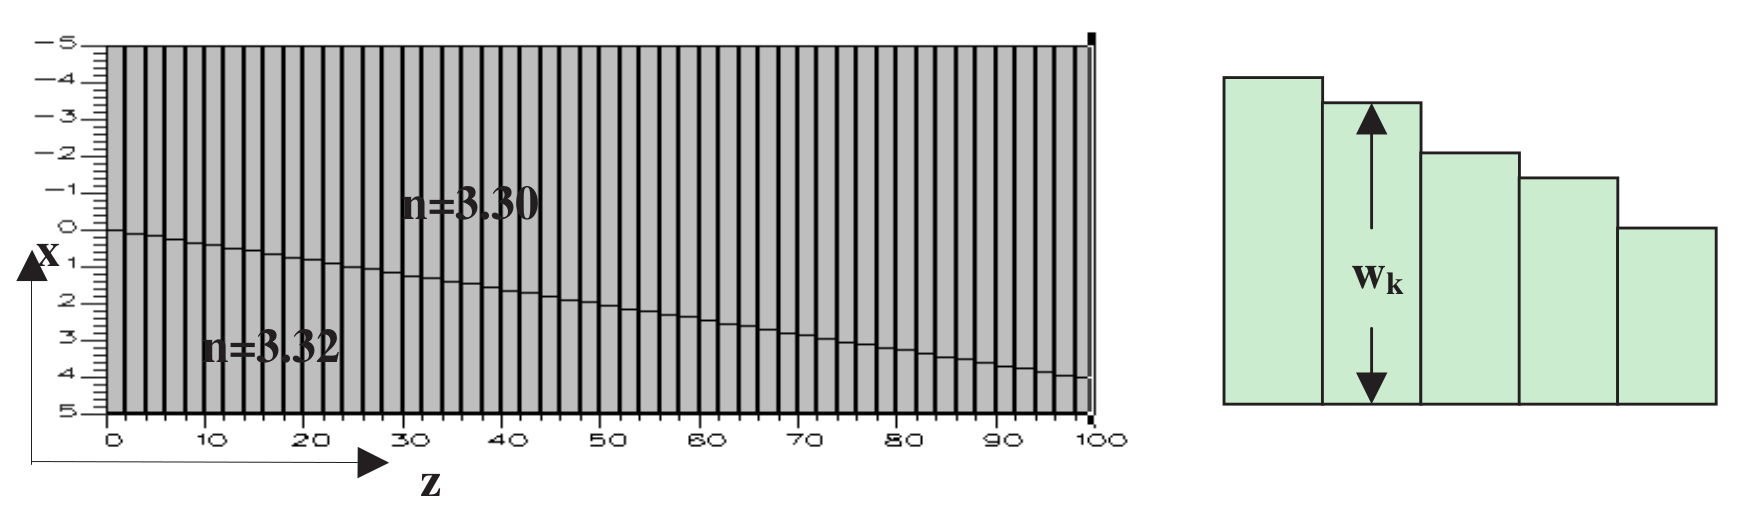
\includegraphics[scale=0.25]{images/numOpti.png}
	\caption{Profil du taper : discrétisation pour le problème d'optimisation}
	\label{fig:numOpti}
\end{figure}

\bigskip
Cette discrétisation impose une régularité très faible pour le profil du taper. On pourrait en effet obtenir des solution avec un profil totalement discontinu. Le champ est calculé grâce à l'analyse faite sur les modes locaux. Les guides d'onde en entrée et en sortie sont choisis tels qu'ils aient au moins un mode guidé. Les dérivées requises sont calculées via un schmé de type différences finies, avec $N=13$ ou $48$ et une solution initiale qui est une droite comme montrée figure \ref{fig:numOpti}.

\subsection{Résultats et interprétation physique}
Les résultats sont assez étonnants : en effet, on pense en général que le profil devrait plutôt ressembler à une courbe assez lisse. Cependant, comme on peut le voir figure \ref{fig:result48}, le résultat n'est pas vraiment ce à quoi on s'attendait. 
\begin{figure}[!h]
	\centering
	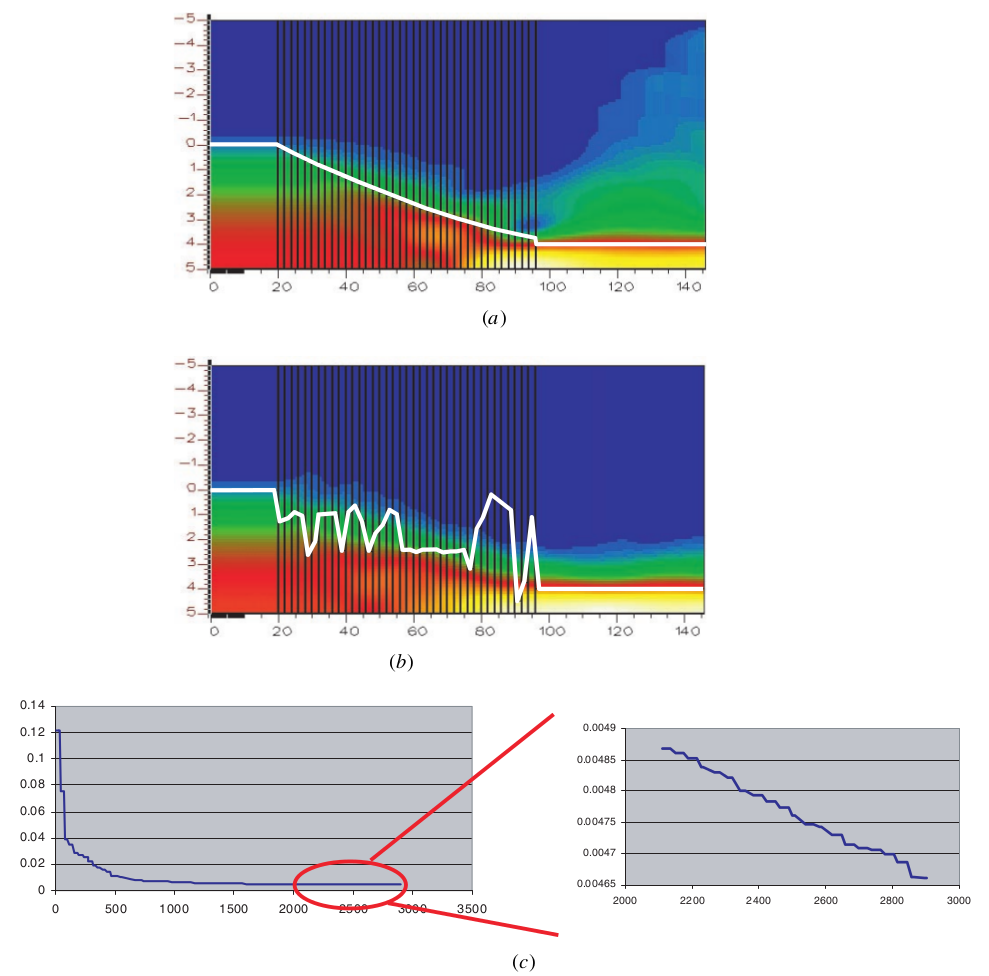
\includegraphics[scale=0.25]{images/result48.png}
	\caption{Profil du taper : résultat avec $N=48$. (a) Forme initial du taper (b) Forme optimale (c) Perte d'énergie en fonction du nombre d'itérations.}
	\label{fig:result48}
\end{figure}
Ces résultats ont été obtenus en 2900 itérations.\\
On remarque dans la figure \ref{fig:powMode} que le mécanisme d'optimisation repose surtout sur une résonnance entre les modes.
\begin{figure}[!h]
	\centering
	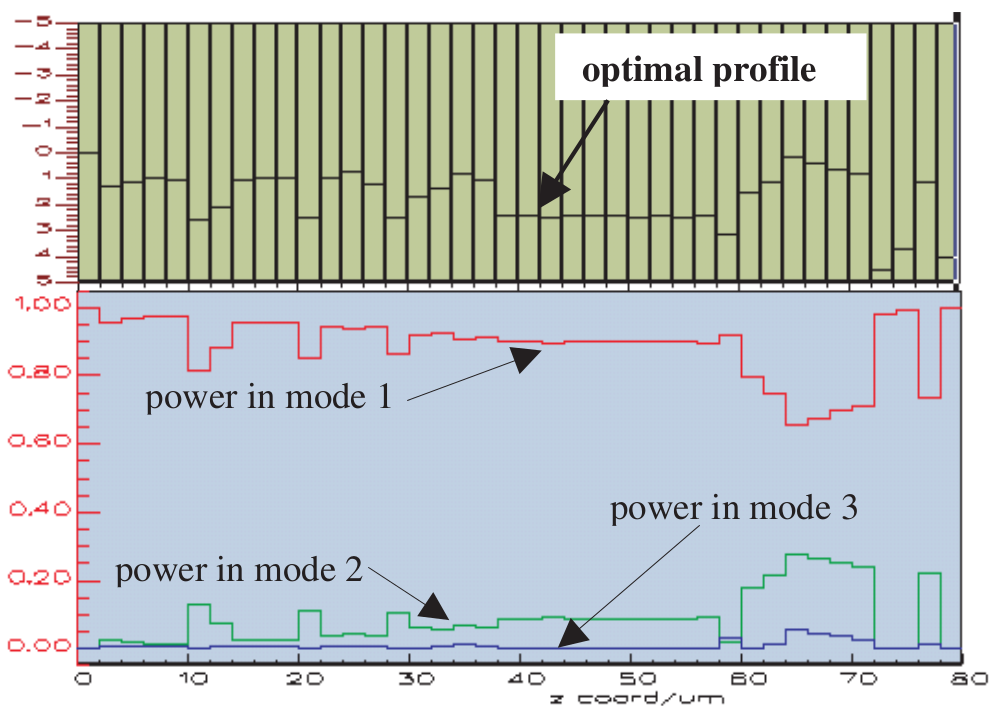
\includegraphics[scale=0.25]{images/powMode.png}
	\caption{L'énergie est préservée grâce à la resonnance avec les autres modes}
	\label{fig:powMode}
\end{figure}
On remarque que le profil est fait de petits pics qui se répètent tous les $10µm$. Cela fait que l'énergie reste presque entièrement dans les deux premiers modes. Après un passage assez plat, le saut final juste avant la fin réintroduit toute la puissance du mode 2 dans le mode 1. La perte d'énergie totale est de seulement 0.5\% en 80µm, tandis qu'un taper plus classique aurait besoin, pour avoir la même efficacité, d'être au moins 5 fois plus long.\\
On ne sait pas, bien sûr, si c'est la solution optimale, mais cette perte d'énergie faible est bien plus importante.\\
Cependant, ces résultats soulèvent une autre problématique : le problème est mal posé.

\subsection{Un problème mal posé}
Les résultats précédents montrent une certaine instabilité au niveau de l'optimisation du profil. Pire encore, cette instabilité semble croître encore avec le nombre de sous-sections $N$.\\
Cela s'explique par le fait qu'on peut toujours trouver une variation arbitrairement grande de la solution qui donnerait toujours un champ $U$ arbitraire assez proche. La solution optimale est donc instable par rapport aux variation de l'indice de réfraction du profil.
On peut voir cela ainsi : supposons que nous avons une solution avec $n^2$ de notre problème d'optimisation, et appliquons une perturbation $\delta n^2$ à $n^2$. Le champ résultant $U$ subira également une perturbation $\delta U$ qui est donné au premier ordre par (\ref{eq10}) :
\begin{equation}\label{eq20}
\begin{array}{l r}
\Delta\delta U + n^2\delta U=-U\delta n^2 & (x,z)\in\Omega\\
\restriction{\delta_U}{\Gamma}=0\\
\frac{\partial \delta U}{\partial z} + i\sum_{k=1}^\infty \beta_k^{(L)}\langle \delta U,\tilde{U}_k^{(L)}\rangle \tilde{U}_k^{(L)} = 0 & \text{ sur }\Gamma_L\\
\frac{\partial \delta U}{\partial z} - i\sum_{k=1}^\infty \beta_k^{(R)}\langle \delta U,\tilde{U}_k^{(R)}\rangle \tilde{U}_k^{(R)} = 0 & \text{ sur }\Gamma_R\\
\end{array}
\end{equation}

Il est souvent utile de réexprimer (\ref{eq20}) sous forme intérgale : on introduit donc la fonction de Green $G(r,r')$ avec $r=(x,z)$ et $r'=(x',z')$.\\
\underline{Fonction de Green :} Si on note $\mathfrak{D}$ un opérateur différentiel linéaire, on note $G(x)$ toute solution de l'équation : 
\[\mathfrak{D} G(x)=\delta(x)\]
où $\delta(x)$ note ici la distribution de Dirac.

\bigskip
Pour en revenir à notre problème, la fonction de Green $G(r,r')$ est exprimée par :
\begin{equation}\label{eq21}
\begin{array}{l r}
\Delta G(r,r')+n(r)^2G(r,r')=\delta(r-r') & r,r'\in\Omega\\
\restriction{G(r,r')}{r\in\Gamma}=0 & r\in\Omega\\
\frac{\partial G(r,r')}{\partial z} + i\sum_{k=1}^\infty \beta_k^{(L)}\langle G,\tilde{U}_k^{(L)}\rangle \tilde{U}_k^{(L)} = 0 & \text{ sur }\Gamma_L\\
\frac{\partial G(r,r')}{\partial z} - i\sum_{k=1}^\infty \beta_k^{(R)}\langle G,\tilde{U}_k^{(R)}\rangle \tilde{U}_k^{(R)} = 0 & \text{ sur }\Gamma_R\\
\end{array}\end{equation}
Le champ $\delta U$ est ainsi donné par l'expresion : 
\[G\Delta\delta U - \delta U\Delta G\equiv \nabla .(G\nabla\delta U - \delta U\nabla G)\]

[... Passage incompris....]

\bigskip
On a donc :
\begin{equation}\label{eq22}
	\delta U(r)=-\int_{r'\in\Omega} G(r,r')U(r')\delta n^2(r')dv := K(\delta n^2)
\end{equation}
C'est une relation intégrale reliant $\delta U$ et $\delta n^2$. Si on considère $\delta U$ donné, (\ref{eq22}) peut être vu comme une équation intégrale (de Fredholm) du premier type pour $\delta n^2$ avec l'opérateur intégral :
\[K : \delta n^2 \mapsto -\int_{z\in\Omega} G(r,r')U(r')\delta n^2(r') dv\]
qui est, en tant qu'opérateur à noyau, compact dans l'espace des fonctions continues $\mathscr{C}^0(\Omega)$. \\
Selon \cite{engl96regu}, les équations intégrale du premier ordre à opérateur compact débouchent sur des problèmes mal posé, dans le sens que pour tout $\delta U$ admissible correspondant à une solution $\delta n^2$, pour tout $\varepsilon$ petit, il existe une autre fonction $\delta n_1^2$ assez éloignée de $\delta n^2$ (mais typiquement, différent de $\delta n^2$ uniquement sur un petit ensemble) tel que $\|K(\delta n_1^2)-\delta U\|<\varepsilon$\\
On en vient donc aux remarques suivantes :
\begin{enumerate}
\item Puisque les fonctions objectifs et les contraintes sur les deux problèmes d'optimisation précédents dépendent explicitement et continuement du champ $U$, et non de l'indice de réfraction $n^2$, de petites variations dans le champ impliquent de petites variation dans les contraintes et les fonctions objectifs. Donc, si $n^2$ est une solution optimale, alors il existe $n_1^2$ aussi éloigné de $n^2$ que l'on veut qui minimise la fonction objectif et qui satisfait également les contraintes à une précision arbitraire.
\item Tout schéma d'optimisation qui utilise d'une quelconque manière la linéarisation précédente pour trouver une direction locale de descente rencontrera des instabilités si on n'ajoute aucune présomption sur l'espace dans lequel on recherche la solution, c'est-à-dire si on cherche une solution optimale $n^2$ dans tout $\mathscr{C}^0(\Omega)$.
\item D'un point de vue physique, ce caractère mal-posé du problème vient du fait que la puissance transmise n'est pas sensible à de grands changements de l'indice de réfraction sur un petit intervalle (comme un pic). En effet, l'onde $U$ "ne voit pas" les variations dans l'indice de réfraction qui sont plus petites que la longueur d'onde de $U$.
\item On pourrait gagner en stabilité en limitant notre recherche à un espace de fonction plus petit. Par exemple, on pourrait chercher la solution optimale $n^2$ dans un sous-ensemble borné de $\mathscr{C}^1(\Omega)$, ce qui éviterait les pics sus-mentionnés. L'équation (\ref{eq22}) deviendrait alors une fonction $K : \mathscr{C}^1(\Omega)\to K(\mathscr{C}^1(\Omega))$ qui aurait un inverse (s'il existe) dans $\mathscr{C}^0(\Omega)$ dû à la compacité de $\mathscr{C}^0(\Omega)$ dans $\mathscr{C}^1(\Omega)$. Si cet inverse n'existe pas, on peut toujours considérer l'inverse généralisé et calculer de manière stable en troncant les valeurs singulières (voir \cite{engl96regu}). Ces considérations seront la base de l'algorithme alternatif décrit juste après.
\end{enumerate}

Pour terminer cette discussion, nous allons discuter le role que joue le fait que ce problème soit mal posé dans ce problème.\\
On considère le problème d'optimisation qui est de trouver une (et pas la) distribution des indices de refraction remplissant un certain nombre de critères. Dans un tel problème, l'uncité n'est pas importante, ni même la stabilité de la solution optimale, puisqu'on souhaite principalement remplir les critères d'optimalité. A contrario, on pourrait aussi considérer le problème inverse, qui est d'identifier la distribution des indices de réfraction provenant d'une certaine mesure. Ce problème inverse est un problème d'identification de paramètre pour une équation aux dérivées partielle et donc mal-posé dans le sens que pour aucune norme disons raisonnable, sa solution (si elle est unique) ne sera pas stable au regard des perturbations sur les données (voir \cite{engl96regu}). Mathématiquement, les deux problèmes sont équivalents - seule la manière de voir le problème est différent. 
On pourrait donc penser que le fait que ce soit mal-posé n'est pas important. Cependant, tout optimiseur digne de ce nom utilisera l'information donnée par le gradient. Comme montré avant, le problème linéarisé à partir duquel on récupère le gradient est en fait mal posé puisqu'il peut être décrit comme une équation intégrale du premier ordre avec un opérateur compact. 
C'est une propriété lié à notre linéarisation, peu importe la manière dont on la résoud, c'est-à-dire même si on n'utilise pas l'intégrale dans notre simulation. Et cela est bien retrouvé dans les simulations !\\
(À voir si on garde...)

\section{L'approche par problème inverse}
Cette approche est basée sur la conservation de la puissance pour (\ref{eq10}), ie :
	\[\mathrm{Im}\int_{z\in\Omega_z} U\frac{\partial \tilde{U}}{\partial z} dx\]
est conservé le long du guide d'onde. Donc la puissance totale doit être la puissance totale à la sortie plus la puissance réfléchie à l'entrée :
\[\begin{array}{l c r}
1=\sum_{k\in RB} |a_{-k}(0)|^2 + \sum_{k\in RB} |a_k(z_R)|^2 &\text{ avec }& RB=\{k\in \mathbb{Z}^* | \beta_k^2>0\}
\end{array}\]
ce qui correspond à la somme sur tous les modes guidés. La seconde somme contient les coefficients de la décomposition spectrale de $U(x,z_r)$ à la sortie du taper :
	\[U(x,z_R)=\sum_{k=1}^\infty a_k(z_R)U_k^{(R)}(x)\]
qui sont déterminés de façon unique par (\ref{eq17}) et (\ref{eq18}) pour un indice de réfraction donné $n$ : dans (\ref{eq18}), tous les coefficients représentant l'onde revenant en arrière ont déjà été mis à 0. Il en suit que la puissance transmise dans le mode fondamental, $|a_1(z_R)|^2$ est toujours plus petit que $1$, et on a égalité uniquement quand :
\begin{equation}\label{eq23}
	\begin{bmatrix} |a_1(z_R)| \\ |a_2(z_R)| \\ |a_3(z_R)| \\ \vdots \end{bmatrix} = \begin{bmatrix} 1 \\ 0 \\ 0 \\ \vdots \end{bmatrix}
\end{equation}
On a donc réexprimé le problème d'optimisation mal posé de minimiser $P(n^2)$ en résolvant (\ref{eq23}) pour l'indice de réfraction inconnu $n$. La dépendance de $U(x,z_R)$ par rapport à $n$ n'est pas linéaire, et il n'existe pas nécessairement de solution de (\ref{eq23}), puisqu'il n'existe pas forcément de profil de longueur finie assurant $P=1$ à la sortie. Cependant, cette formulation a l'avantage numérique qu'on prend également en compte $a_2$, $a_3$,... en plus de $a_1$. Même si ce n'est pas nécessaire, cela devrait aider numériquement à "attirer" ces coefficients vers les bonnes valeurs en résolvant (\ref{eq23}) au sens des moindes carrés. On utilisera pour cela une approche du type méthode de Newton.\\
On réécrit (\ref{eq23}) $\mathbf{a}(n)=\mathbf{a}_1$ avec \[\mathbf{a}_1=\begin{bmatrix} 1\\0\\0\\ \vdots \end{bmatrix} \ \mathbf{a}(n)=\begin{bmatrix} |a_1(z_R)| \\ |a_2(z_R)| \\ |a_3(z_R)| \\ \vdots \end{bmatrix}\]
Pour simplifier l'écriture, on va omettre les carrés sur $n^2$ et $\delta n^2$. Une étape dans la méthode de Newton donnant la prochaine itération $n+\delta n$ depuis $n$ est donné par le problème linéaire :
\begin{equation}\label{eq24}
	\restriction{\frac{\partial\mathbf{a}}{\partial n}}{n}\delta n=\mathbf{a}_1-\mathbf{a}(n)
\end{equation}
En paramétrisant $n$ pour les $N$ sous-sections, $\restriction{\frac{\partial\mathbf{a}}{\partial n}}{n}$ est une matrice $M\times N$, où $M$ est l'indice du dernier mode retenu.\\
Ce jacobien a été calculé en utilisant un schéma de type différences finies. Notons que selon le choix de $M$ et $N$, le système peut être sous- ou sur-déterminé, mais il sera de toute façon résolu au sens des moindres carrés. Cependant, plus on augmente $M$, plus la solution sera instable, étant donné qu'il s'agit de la discrétisation d'un problème mal-posé. On pourrait utiliser pour régler ce problème des méthodes de régularisation de la théorie des problèmes inverses (voir \cite{engl96regu}), mais il a été choisi ici d'utiliser une méthode heuristique de régularisation basé une troncature des valeurs singulières.\\
Résoudre (\ref{eq24}) par les moindres carrés peut être fait un faisant une décomposition en valeurs singulières du Jacobien ;
	\[\restriction{\frac{\partial\mathbf{a}}{\partial n}}{n}=UDV^T\]
où $U$ et $V$ sont des matrices unitaires et $D$ une matrice diagonale avec les valeurs singulières en diagonale suivie de zéros. On note $d_k$, $k\leq \min(M,N)$ ces valeurs singulières, et on les suppose rangées : $d_1\geq d_2\geq \cdots \geq d_k$. Étant donné qu'on part d'une disrétisation, on s'attend à ce que les plus petites valeurs singulières décroissent vers 0 si la dimension de la matrice augmente.\\
La régularisation consiste en la troncature des petites valeurs singulières : on choisit un paramètre de régularisation $0<\alpha<1$ et on pose :
	\[r:=\max\{i | d_i\geq \alpha d_1\}\]
Et :
	\[D_{red}=diag(d_1,...,d_r,0,...,0)\]
d'inverse généralisé :
	\[D_{red}^\dagger = diag\left( \frac{1}{d_1},...,\frac{1}{d_r},0,...,0\right) \]
L'étape $\delta n$ est donc choisi comme : \begin{equation}\label{eq26}
	\delta n=VD_{red}^\dagger U^\dagger [\mathbf{a}_1-\mathbf{a}(n)]
\end{equation}

(Revoir direction de descente)

\section{Simulation numérique utilisant l'approche problème inverse}
L'algorithme utilisé est le suivant : étant donné une étape $n_k$ donné, la prochaine itération est donné par (\ref{eq26}). On cherche ensuite à minimiser :
	\[F(\lambda)=\|\mathbf{a}_1-\mathbf{a}(n_k+\lambda\delta n\|_2^2\]
et on pose
	\[n_{k+1}=n_k+\lambda_{min}\delta n\]
On répète ce processus jusqu'à ce que $\|\mathbf{a}_1-\mathbf{a}(n)\|_2$ arrête de décroître.\\
Pour comparer les deux algorithmes (entre la méthode directe et l'approche problème inverse), les deux algorithmes sont lancés avec le même nombre d'itérations, et la puissance à la fin de ces itérations est enfin comparée.\\
On remarque d'abord une forte variation en fonction du paramètre de régularisation $\alpha$ choisi. Il semble y avoir, pour $N=13$ et $N=48$ à chaque fois une région pour $\alpha$ où l'algorithme semble mieux fonctionner. Cela se comprend aisément :
\begin{itemize}
	\item Si le paramètre est trop proche de 1, seuls les valeurs singulières trop hautes sont retenues, et donc la correction $\delta n$ sera toujours d'autant plus douce. Cependant, comme on peut le voir sur les simulations, la solution semble bien être très irrégulière. La convergence semble donc être ralentie par les corrections trop faibles apportées à chaque fois.
	\item A contrario, un paramètre trop proche de zéro retiendra des valeurs singulières très petite, et augmentera d'autant plus l'instabilité numérique.
\end{itemize}

Dueixème chose : pour un choix raisonnable du paramètre $\alpha$, les deux algorithmes donnent des résultats similaires dans le cas d'une discrétisation assez grossière, mais la méthode en problème inverse devient plus intéressant pour des discrétisations plus fines (comme on peut le voir figure \ref{fig:accConv}). Cela montre que la régularisation peut en effet accélérer la convergence et nous permettre d'obtenir des résultats en un temps raisonnable, ce qui ne serait pas réalisable avec la l'algorithme direct. 
\begin{figure}[!h]
	\centering
	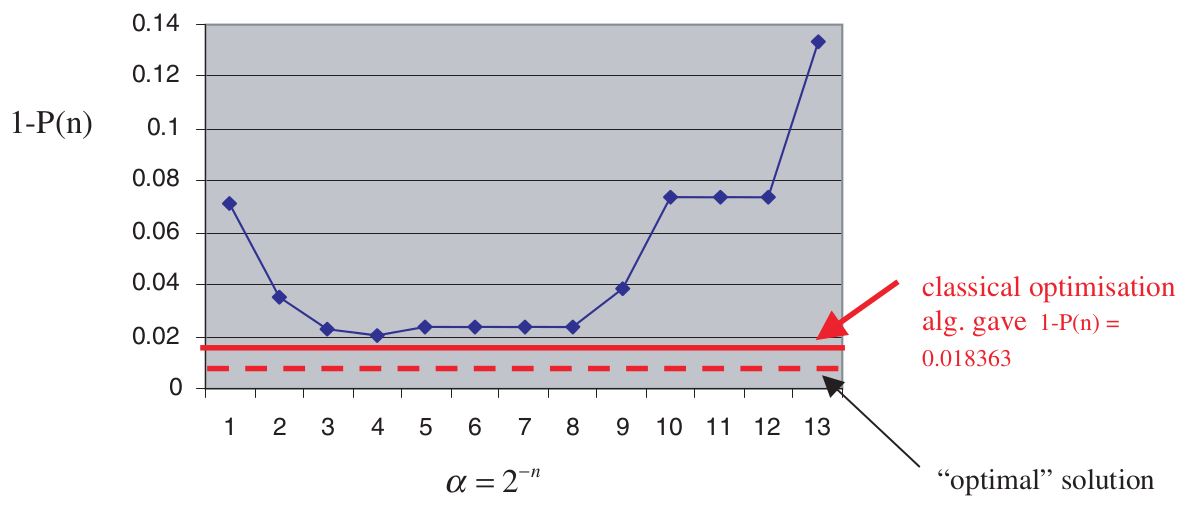
\includegraphics[scale=0.35]{images/convAlgo13.png}
	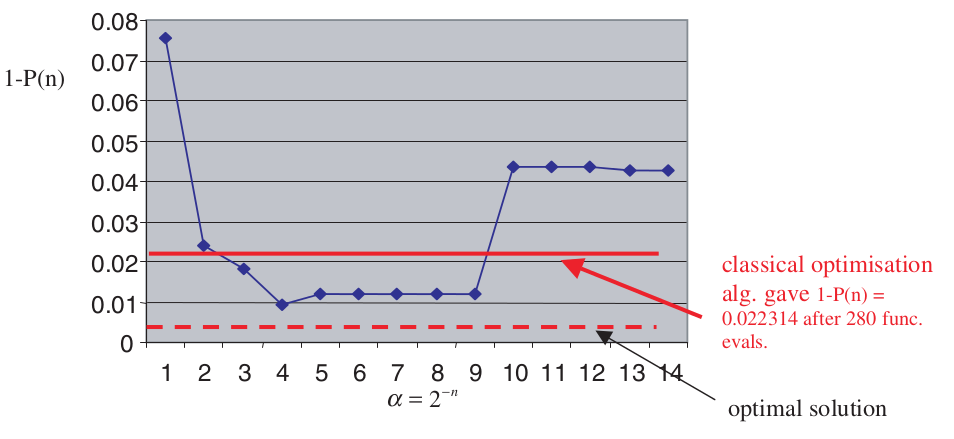
\includegraphics[scale=0.35]{images/convAlgo48.png}
	\caption{Convergence des deux algorithmes : premier cas avec 13 sous-sections et 10 modes, deuxième cas avec 48 sous-sections et 15 modes}
	\label{fig:accConv}
\end{figure}

\section{Algorithme en cascade}
Malgré le fait que le problème soit mal posé, on peut tout de même utiliser le problème direct et le même optimiseur pour trouver une solution intéressante.\\
L'idée est simple : on commence avec une discrétisation grossière pour avoir un optimum approché. On redivise ensuite le profil en subdivisions plus fines, et on prend comme solution initiale celle trouvée précédemment (en interpolant quelque peu les données pour correspondre à ce nouveau maillage). On note d'ailleurs qu'on peut même augmenter la vitesse de calcul en limitant (du moins pour les premières recherches d'optimum) le nombre de modes, puis qu'ils ne serviront qu'à avoir une solution initiale à l'itération d'après. Notons également que si on utilise l'agorithme par la méthode inverse, il faudra également décroître le paramètre $\alpha$ à chaque rafinement.\\
\begin{figure}[!h]
	\centering
	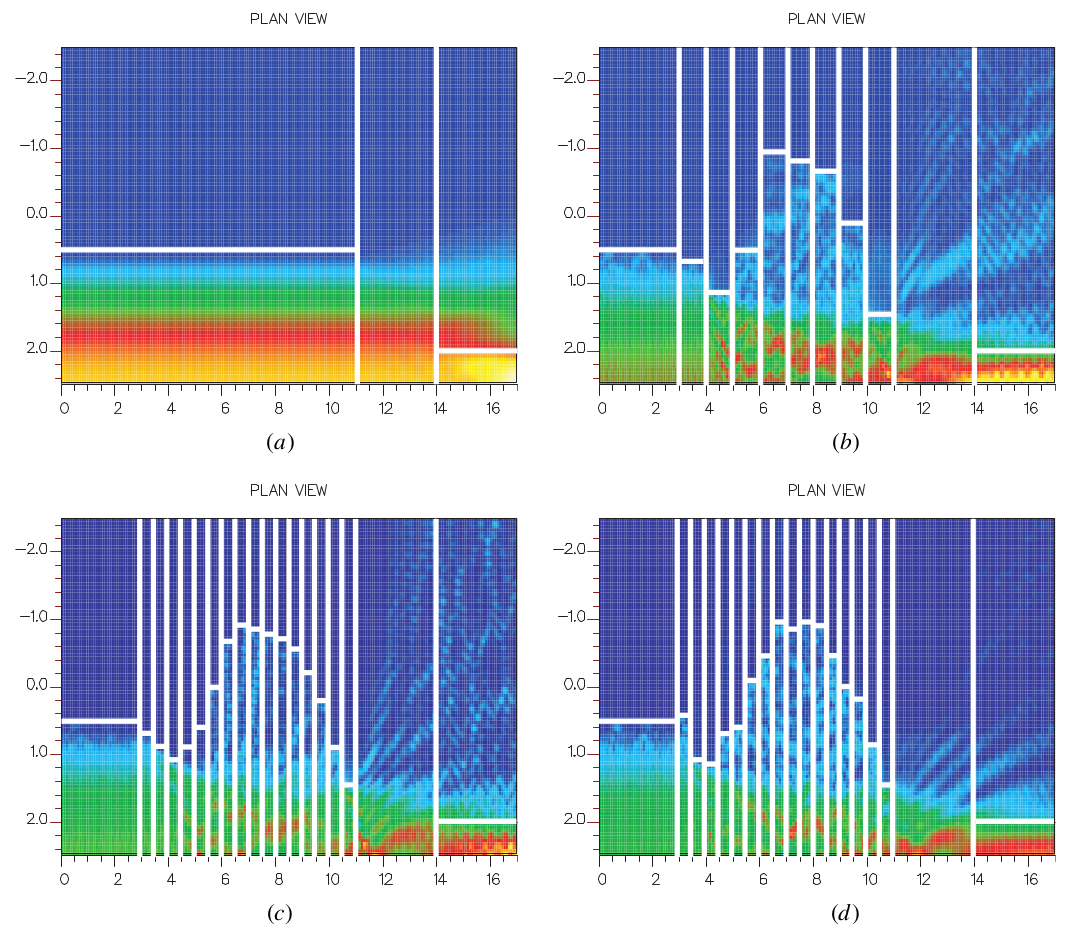
\includegraphics[scale=0.35]{images/cascade.png}
	\caption{(a) Solution initiale (b) Solution grossière (c) Rafinement et interpolation de la solution grossière (d) Solution avec le rafinement}
	\label{fig:cascade}
\end{figure}
L'exemple montré figure \ref{fig:cascade} utilise ce procédé. Il fallait maximiser la puissance transmise par un guide d'onde où la sortie (beaucoup plus petite) est placée à une certaine distance (non nulle) du guide d'onde, et séparé par un milieu vide. La solution ressemble à une lentille, ce qui est attendu. 

\bibliographystyle{plain}
\bibliography{bibliographie}
\end{document}
